\documentclass[12pt]{article}
\usepackage{e-jc}
\usepackage[colorlinks=true,citecolor=black,linkcolor=black,urlcolor=blue]{hyperref}
\usepackage{
	amsmath,
	amssymb,
	amsthm,
	array,caption,
	chngpage,float,graphicx,
	mathrsfs,
	multicol,multirow,numprint,rotating,sectsty,
	spreadtab,subcaption,
	tikz,
	url,
	verbatim,
	wrapfig
}
\usetikzlibrary{automata, positioning}

\newcommand{\eps}{\varepsilon}
\newcommand{\squarefree}{square-free}
\newcommand{\cubefree}{cube-free}
\newcommand{\Squarefree}{Square-free}
\newcommand{\Cubefree}{Cube-free}
\newcommand{\abs}[1]{\lvert#1\rvert}
\newcommand{\myUrl}[1]{
	\begin{center}
		{\small\url{#1}} 
	\end{center}
}

\theoremstyle{plain}
\newtheorem{thm}{Theorem}
\newtheorem{cor}[thm]{Corollary}
\newtheorem{lem}[thm]{Lemma}
\newtheorem{pro}[thm]{Proposition}

\theoremstyle{definition}
\newtheorem{df}[thm]{Definition}
\newtheorem{exa}[thm]{Example}
\newtheorem{con}[thm]{Conjecture}

\theoremstyle{remark}
\newtheorem{rem}[thm]{Remark}

\DeclareMathOperator{\first}{first}
\DeclareMathOperator{\last}{last}
\title{
	Nondeterministic automatic complexity of overlap-free and almost {\squarefree} words
}

\author{Kayleigh K. Hyde\\
\small Schmid College of Science \& Technology\-0.8ex] 
\small Orange, California, U.S.A.\\
\small\tt khyde@chapman.edu\\
\and
Bj{\o}rn Kjos-Hanssen\thanks{This work was partially supported by a grant from the Simons Foundation (\#315188 to Bj\o rn Kjos-Hanssen).}\\
\small Department of Mathematics\-0.8ex]
\small Honolulu, Hawai\textquoteleft i, U.S.A.\\
\small\tt bjoernkh@hawaii.edu\\
}

\date{
	\dateline{November 24, 2014}{July 29, 2015}\\
	\small Mathematics Subject Classifications: 68R15, 68Q30
}


\begin{document}
	\maketitle{}
	\begin{abstract}
		Shallit and Wang studied deterministic automatic complexity of words. 
		They showed that the automatic Hausdorff dimension  of the infinite Thue word satisfies .
		We improve that result by showing that .
		We prove that the nondeterministic automatic complexity  of a word  of length  is bounded by .
		This enables us to define the complexity deficiency .
		If  is square-free then . If  is almost square-free in the sense of Fraenkel and Simpson,
		or if  is a overlap-free binary word such as the infinite Thue--Morse word, then .
		On the other hand, there is no constant upper bound on  for overlap-free words over a ternary alphabet,
		nor for cube-free words over a binary alphabet.
		
		
		
		The decision problem whether  for given ,  belongs to .
	\end{abstract}

	\section{Introduction}
		The Kolmogorov complexity of a finite word  is, roughly speaking,
		the length of the shortest description  of  in a fixed formal language.
		The description  can be thought of as an optimally compressed version of .
		Motivated by the non-computability of Kolmogorov complexity,
		Shallit and Wang \cite{MR1897300} studied a deterministic finite automaton analogue.
		A more recent approach is due to Calude, Salomaa, and Roblot \cite{Calude}.

		\begin{df}[Shallit and Wang \cite{MR1897300}]
			The \emph{automatic complexity} of a finite binary string  is 
			the least number  of states of a {deterministic finite automaton}  such that 
			 is the only string of length  in the language accepted by .
		\end{df}
		This complexity notion has the following two properties:
		\begin{enumerate}
			\item{} Most of the relevant automata end up
				having a ``dead state'' whose sole purpose is to absorb any irrelevant or
				unacceptable transitions.
			\item{} The complexity of a string can be changed by reversing it. For instance,
				
			Equation \ref{eq1} was verified by a computer program; for the idea and a partial proof see Figure \ref{referee}.
			The anonymous referee of this article raised the question, which we have not been able to answer,
			whether the complexity of a string and its reverse can be arbitrarily far apart.
		\end{enumerate}

		\begin{figure}
			\begin{center}
				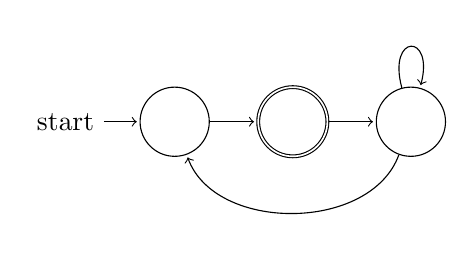
\begin{tikzpicture}[shorten >=1pt,node distance=1.5cm,on grid,auto]
					\node[state,initial]   (q_0)                {};
					\node[state,accepting] (q_1) [right of=q_0] {};
					\node[state]           (q_2) [right of=q_1] {};
					\path[->] 
						(q_0) edge                node {} (q_1)
						(q_1) edge                node {} (q_2)
						(q_2) edge [loop above]   node {} ()
						(q_2) edge [bend left=70] node {} (q_0);
				\end{tikzpicture}
			\end{center}
			\caption{A witnessing automaton for the inequality .
				All missing transitions go to a dead state  which is not shown.
			}\label{referee}
		\end{figure}

		If we replace {deterministic finite automata} by {nondeterministic} ones, these properties disappear.
		The nondeterministic automatic complexity turns out to have other pleasant properties, such as a sharp linear upper bound.
		\paragraph{Technical ideas and results.} In this paper we develop some of the properties of nondeterministic automatic complexity.
		As a corollary we get a strengthening of a result of Shallit and Wang \cite{MR1897300}
		on the complexity of the infinite Thue--Morse word .
		Moreover, viewed through an NFA lens we can, in a sense, characterize the complexity of  exactly.
		A main technical idea is to extend \cite[Theorem 9]{MR1897300} which said that
		not only do squares, cubes and higher powers of a word have low complexity,
		but a word completely free of such powers must conversely have high complexity.
		The way we strengthen their results is by considering a variation
		on square-freeness and cube-freeness, \emph{overlap-freeness}.
		This notion also goes by the names of \emph{irreducibility} and \emph{strong cube-freeness} in the combinatorial literature.
		We also take up an idea from \cite[Theorem 8]{MR1897300} and use it to show that
		the natural decision problem associated with nondeterministic automatic complexity is in E = DTIME().
		This result is a theoretical complement to the practical fact that
		the nondeterministic automatic complexity can be computed reasonably quickly;
		to see it in action, for strings of length up to 23
		one can view automaton witnesses and check complexity using the following URL format
			\myUrl{http://math.hawaii.edu/wordpress/bjoern/complexity-of-110101101/}
		and check one's comprehension by playing a Complexity Guessing Game at
			\myUrl{http://math.hawaii.edu/wordpress/bjoern/software/web/complexity-guessing-game/}
		Let us now define our central notion and get started on developing its properties.
		Recall that a nondeterministic finite automaton (NFA) is assumed to have no -transitions, i.e.,
		it is not an .
		\begin{df}\label{precise}
			The nondeterministic automatic complexity  of a word  is the minimum number of states of an NFA  accepting 
			such that there is only one accepting path in  of length .
		\end{df}
		The minimum complexity  is only achieved by words of the form  where  is a single letter.
		\begin{thm}[Hyde \cite{Hyde}]\label{Hyde}
			The nondeterministic automatic complexity  of a string  of length  satisfies
			
		\end{thm}
		\begin{proof}[Proof sketch.]
			If  has odd length, it suffices to carefully consider the automaton in Figure \ref{fig1}.
			If  has even length, a slightly modified automaton can be used.
		\end{proof}
		\begin{figure}[h]
			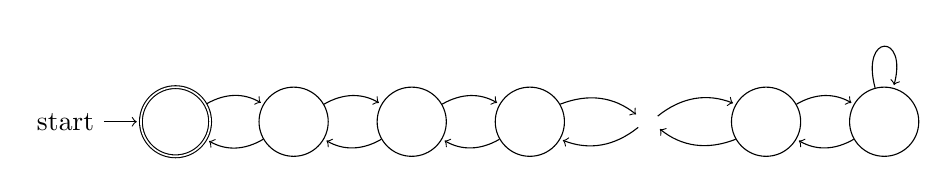
\begin{tikzpicture}[shorten >=1pt,node distance=1.5cm,on grid,auto]
				\node[state,initial, accepting] (q_1)   {}; 
				\node[state] (q_2)     [right=of q_1   ] {}; 
				\node[state] (q_3)     [right=of q_2   ] {}; 
				\node[state] (q_4)     [right=of q_3   ] {};
				\node        (q_dots)  [right=of q_4   ] {};
				\node[state] (q_m)     [right=of q_dots] {};
				\node[state] (q_{m+1}) [right=of q_m   ] {}; 
				\path[->] 
					(q_1)     edge [bend left]  node           {}     (q_2)
					(q_2)     edge [bend left]  node           {}     (q_3)
					(q_3)     edge [bend left]  node           {}     (q_4)
					(q_4)     edge [bend left]  node [pos=.45] {}     (q_dots)
					(q_dots)  edge [bend left]  node [pos=.6]  {} (q_m)
					(q_m)     edge [bend left]  node [pos=.56] {}     (q_{m+1})
					(q_{m+1}) edge [loop above] node           {} ()
					(q_{m+1}) edge [bend left]  node [pos=.45] {} (q_m)
					(q_m)     edge [bend left]  node [pos=.4]  {} (q_dots)
					(q_dots)  edge [bend left]  node [pos=.6]  {} (q_4)
					(q_4)     edge [bend left]  node           {} (q_3)
					(q_3)     edge [bend left]  node           {} (q_2)
					(q_2)     edge [bend left]  node           {}     (q_1);
			\end{tikzpicture}
			\caption{
				A nondeterministic finite automaton that only accepts one string
				 of length .
			}
			\label{fig1}
		\end{figure}


		\begin{df}
			The \emph{complexity deficiency} of a word  of length  is
			
		\end{df}
		The distribution of  for  of length  is given in Table \ref{deficiency}.
		The notion of deficiency is motivated by the experimental observation that about half of all strings have deficiency 0.
		\begin{sidewaystable}
			\centering
			\begin{spreadtab}{{tabular}{|r|r|r|r|r|r|r|r|r|r|r|r|r|}}
				\hline
				@ &1&2&3&4&5&6&7&8&9&10&11&12\\
				\hline
23 & :={8388608-sum(c2:m2)} & 6 & 20 & 58 & 164 &  430 & 2540 & 14252 &  80962 & 442278 & 2160662 & 5687234\\
				22 & :={4194304-sum(c3:m3)} & 6 & 20 & 58 & 164 &  502 & 2846 & 16024 &  94732 & 451368 & 2089418 & 1539164\\
				21 & :={2097152-sum(c4:m4)} & 6 & 20 & 58 & 176 &  496 & 3168 & 18720 & 108042 & 504794 & 1461670 &\\
				20 & :={1048576-sum(c5:m5)} & 6 & 20 & 58 & 164 &  430 & 3814 & 23328 & 115896 & 529148 &  375710 &\\
				19 &  :={524288-sum(c6:m6)} & 6 & 20 & 58 & 164 &  582 & 4996 & 26542 & 140668 & 351250 & &\\
				18 &  :={262144-sum(c7:m7)} & 6 & 20 & 58 & 188 &  598 & 5692 & 29990 & 136024 &  89566 & &\\
				17 &  :={131072-sum(c8:m8)} & 6 & 20 & 58 & 200 &  514 & 7102 & 37042 &  86128 & &&\\
				16 &   :={65536-sum(c9:m9)} & 6 & 20 & 58 & 164 &  752 & 7738 & 34320 &  22476 & &&\\
				15 & :={32768-sum(c10:m10)} & 6 & 20 & 58 & 226 &  908 & 8530 & 23018 & &&&\\
				14 & :={16384-sum(c11:m11)} & 6 & 20 & 58 & 244 & 1270 & 9668 &  5116 & &&&\\
				13 &  :={8192-sum(c12:m12)} & 6 & 20 & 64 & 250 & 2076 & 5774 &       & &&&\\
				12 &  :={4096-sum(c13:m13)} & 6 & 20 & 58 & 282 & 2090 & 1638 &       & &&&\\
				11 &  :={2048-sum(c14:m14)} & 6 & 20 & 58 & 564 & 1398 &      &       & &&&\\
				10 &  :={1024-sum(c15:m15)} & 6 & 20 & 64 & 588 &  344 &      &       & &&&\\
				 9 &   :={512-sum(c16:m16)} & 6 & 20 & 78 & 406 &      &      &       & &&&\\
				 8 &   :={256-sum(c17:m17)} & 6 & 20 & 130&  98 &      &      &       & &&&\\
				 7 &   :={128-sum(c18:m18)} & 6 & 22 & 98 &     &      &      &       & &&&\\
				 6 &    :={64-sum(c19:m19)} & 6 & 26 & 30 &     &      &      &       & &&&\\
				 5 &    :={32-sum(c20:m20)} & 6 & 24 &    &     &      &      &       & &&&\\
				 4 &    :={16-sum(c21:m21)} & 6 &  8 &    &     &      &      &       & &&&\\
				 3 &     :={8-sum(c22:m22)} & 6 &    &    &     &      &      &       & &&&\\
				 2 &     :={4-sum(c23:m23)} & 2 &    &    &     &      &      &       & &&&\\
				 1 &     :={2-sum(c24:m24)} &   &    &    &     &      &      &       & &&&\\0 & 1                      &   &    &    &     &      &      &       & &&&\\
				\hline
			\end{spreadtab}
			\caption{The number of strings of length  having nondeterministic automatic complexity .}\label{deficiency}
		\end{sidewaystable}
	\section{Time complexity}
		\begin{df}
			Let \textsc{DEFICIENCY} be the following decision problem.

			\emph{Given a binary word  and an integer , is ?}
		\end{df}
		\subsection{NP}
			Theorem \ref{np} is not surprising; we do not know whether \textsc{DEFICIENCY} is -complete.
			\begin{thm}\label{np}
				\textsc{DEFICIENCY} is in .
			\end{thm}
			\begin{proof}
				Shallit and Wang \cite[Theorem 2]{MR1897300} showed that
				one can efficiently determine whether a given DFA uniquely accepts  among string of length .
				Hyde \cite[Theorem 2.2]{Hyde} extended that result to NFAs, from which the result easily follows.
			\end{proof}
		\subsection{E}
			\begin{df}
				Suppose  is an NFA with  states that uniquely accepts a word  of length .
				Throughout this paper we may assume that  contains no edges except those
				traversed on input .
				Consider the \emph{almost unlabeled transition diagram} of , which is
				a directed graph whose vertices are the states of 
				and whose edges correspond to transitions.
				Each edge is labeled with a 0 except for an edge entering the initial state as described below.

				We define the \emph{accepting path}  for  to be the sequence of  edges traversed in this graph,
				where we include as first element an edge labeled with the empty string  that enters the initial state  of .

				We define the \emph{abbreviated accepting path}  to be the sequence of edges obtained from  by considering each edge
				in order and deleting it if it has previously been traversed.
			\end{df}
			\begin{lem}\label{types}
				Let  be a vertex visited by an abbreviated accepting path .
				Then  is of one of the following five types.
				\begin{enumerate}
					\item In-degree 1 (edge ), out-degree 1 (edge ).
					\item In-degree 2 (edges  and  with ), out-degree 1 ().
					\item In-degree 1 (edge ), out-degree 2 (edges  and , ).
					\item In-degree 2 (edges  and  with ), out-degree 2 ( and ).
					\item In-degree 1 (edge ), out-degree 0.\footnote{This type was omitted by Shallit and Wang.}
				\end{enumerate}
			\end{lem}
			\begin{proof}
				The out-degree and in-degree of each vertex encountered along  are both ,
				since failure of this would imply non-uniqueness of accepting path.
				Since all the edges of  are included in , the list includes all the possible in-degree, out-degree combinations.
				We can define  by the rule that  is the first edge in  entering .
				Again, since all the edges of  are included in ,
				 must be one of the edges contributing to the out-degree of , if any,
				and  must also be as specified in the types.
			\end{proof}
			Lemma \ref{types} implies that Definition \ref{def:E} makes sense.
			\begin{df}\label{def:E}
				For  and  we let  be a string representing the edges .
				The meaning of the symbols is as follows: 0 represents an edge.
				A left bracket  represents a vertex that is the target of a backedge.
				A right bracket  represents a backedge.
				The symbol  represents a vertex of out-degree 2.
				When , we set .
				Next, assuming we have defined  for all  and all ,
				we can define  by considering the type of the vertex reached by the edge .
				Let  be the label of .
				\begin{enumerate}
					\item{} .
					\item{} .
					\item{} .
					\item{} .
					\item{} .
				\end{enumerate}
			\end{df}
			\begin{figure}
				\begin{subfigure}[b]{0.5\textwidth}
					\centering \begin{tabular}{|c|c|}
						\hline{}
						&Computation\\
						\hline{}
						 & \\
						 & \\
						 & \\
						 & \\
						 & \\
						 & \\
						 & \\
						 & \\
						 & \\
						 & \\
						 & \\
						 & \\
						 & \\
						 & \\
						 & \\
						\hline
					\end{tabular}
					\caption{
						The  marks the place of a loopback.
					}
					\label{computation}
				\end{subfigure}
				\begin{subfigure}[b]{0.1\textwidth}
				\end{subfigure}
				\begin{subfigure}[b]{0.4\textwidth}
					\centering 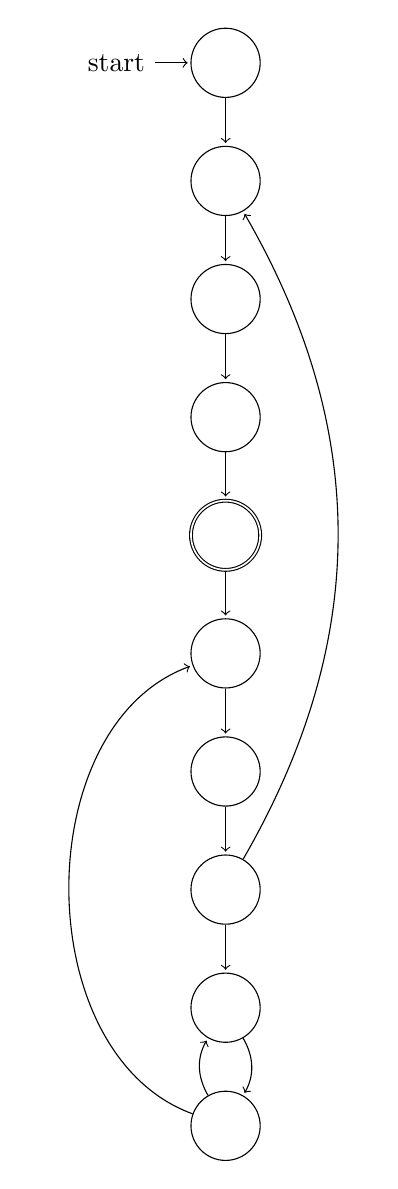
\begin{tikzpicture}[shorten >=1pt,node distance=1.5cm,on grid,auto]
						\node[state,initial]   (q_0)                {}; 
						\node[state]           (q_1) [below of=q_0] {}; 
						\node[state]           (q_2) [below of=q_1] {}; 
						\node[state]           (q_3) [below of=q_2] {};
						\node[state,accepting] (q_4) [below of=q_3] {};
						\node[state]           (q_5) [below of=q_4] {};
						\node[state]           (q_6) [below of=q_5] {};
						\node[state]           (q_7) [below of=q_6] {};
						\node[state]           (q_8) [below of=q_7] {};
						\node[state]           (q_9) [below of=q_8] {};
						\path[->] 
							(q_0) edge              node {} (q_1)
							(q_1) edge              node {} (q_2)
							(q_2) edge              node {} (q_3)
							(q_3) edge              node {} (q_4)
							(q_4) edge              node {} (q_5)
							(q_5) edge              node {} (q_6)
							(q_6) edge              node {} (q_7)
							(q_7) edge              node {} (q_8)
							(q_8) edge [bend left]  node {} (q_9)
							(q_9) edge [bend left]  node {} (q_8)
							(q_9) edge [bend left=70]  node {} (q_5)
							(q_7) edge [bend right] node {} (q_1);
					\end{tikzpicture}
					\caption{
						Complexity witness for the string 0100011001010101111100, one of the 2,655,140 simple strings of length .}
				\end{subfigure}
				\caption{
					The code is
						
					where
					. In reduced form, 
						.
				}\label{fig:Figure3}
			\end{figure}
			\begin{lem}\label{reconstructed}
				The abbreviated accepting path can be reconstructed from .
			\end{lem}
			We do not include the proof of Lemma \ref{reconstructed};
			instead, Figure \ref{fig:Figure3} gives an example of an automaton and the computation of .
			\begin{lem}\label{easy}
				
			\end{lem}
			\begin{proof}[Proof of Lemma \ref{easy}.]
				The four rules are
				\begin{enumerate}
					\item{} 
					\item{} 
					\item{} 
					\item{} 
				\end{enumerate}
				So either
				
				or
				
				So if by induction hypothesis  then
				
				or
				
			\end{proof}
			\begin{thm}\label{singly}
	 			\textsc{DEFICIENCY} is in E.
			\end{thm}
			\begin{proof}
				Let  be a word of a length , and let . To determine whether ,
				we must determine whether there exists an NFA  with at most  states
				which accepts , and accepts no other word of length .
				Since there are \emph{prima facie} more than single-exponentially many automata to consider,
				we consider instead codes  as in Definition \ref{def:E}.
				By Lemma \ref{reconstructed} we can recover the abbreviated accepting path  and hence  from such a code.
				The number of edges  is bounded by the string length , so by Lemma \ref{easy}
				
				since there are four symbols this gives
				
				codes to consider.
				Finally, to check whether a given  accepts uniquely takes only polynomially many steps, as in Theorem \ref{np}.
			\end{proof}
			\begin{rem}
				The bound  counts many automata that are not uniquely accepting; the actual number may be closer to  based on
				computational evidence.
			\end{rem}

	\section{Powers and complexity}
		In this section we shall exhibit infinite words all of whose prefixes have complexity deficiency bounded by 1.
		We say that such a word has a hereditary deficiency bound of 1.
		\subsection{{\Squarefree} words}
			\begin{lem}\label{lyndon:schuetzenberger}
				Let  and  be strings over an arbitrary alphabet with .
				Then there is a string  and integers  and  such that  and .
			\end{lem}
			Lemma \ref{lyndon:schuetzenberger} is proved in Shallit \cite[Theorem 2.3.3]{Shallit:2008:SCF:1434864}
			and is originally due to Lyndon and Schuetzenberger \cite{MR0162838}.
			\begin{df}\label{factor}
				A word  is a \emph{factor} in a word  if  for some words  and .
				In this case we also say that  \emph{contains} .
			\end{df}

			We will use the following simple strengthening from DFAs to NFAs of a fact used in \cite[Theorem 9]{MR1897300}.
			\begin{thm}\label{nfa9fact}
				If an NFA  uniquely accepts  of length , and visits a state  at least  times, where ,
				during its computation on input ,
				then  contains a th power.
			\end{thm}
			\begin{proof}
				Let  where
				\begin{itemize}
					\item  is the portion of  read before the first visit to the state ,
					\item  is the portion of  read between visits number  and  to the state  for , and
					\item  is the portion of  read after the last visit to the state .
				\end{itemize}
				Thus  for each , but it is possible to have  () since the
				initial (final) state of 's on input  computation may be .

				For any permutation  on ,  accepts .
				Let  be such that  has minimal length and let
				
				Then  also accepts
				
				By uniqueness,
				
				and so
				
				By Lemma \ref{lyndon:schuetzenberger},  and  are both powers of a string .
				Since ,  is at least a th power of , so  contains a th power of .
			\end{proof}
			\begin{thm}[Extended Pigeonhole Principle]\label{php}
				If  pigeons are placed in  pigeonholes where ,
				then it cannot be the case that all pigeonholes have at most  pigeons;
				in fact, either
				\begin{itemize}
					\item{} there is a pigeonhole with at least  pigeons; or
					\item{} there is a pigeonhole with at least  pigeons, and another with  pigeons; or
					\item{} there is a pigeonhole with at least  pigeons, and another with  pigeons; or		
					\item{} there is a pigeonhole with at least  pigeons, and two others with  pigeons; or
					\item{} all pigeonholes have at most  pigeons (which is impossible if  and ).
				\end{itemize}
			\end{thm}
			\begin{proof}
				Consider the maximum number of pigeons in a pigeonhole . If  we are in Case 1.
				If , we consider all the other pigeons and pigeonholes;
				there are then  pigeonholes and  pigeons.
				By the plain Pigeonhole Principle, there is a pigeonhole with at least  pigeons.
				If , we repeat the argument,
				consider the maximum number of pigeons in a pigeonhole other than a given one with the maximum number
				of pigeons.
			\end{proof}
			We next strengthen a particular case of \cite[Theorem 9]{MR1897300} to NFAs.
			\begin{thm}\label{nfa9square}
				A {\squarefree} word has deficiency 0.
			\end{thm}
			\begin{proof}
				Suppose  is a word of length  or , of deficiency .
				Then there is a witnessing automaton  with  states.
				Since , by the Extended Pigeonhole Principle (Theorem \ref{php}),
				there is a state  which is visited  times , during the  times of the computation of 
				on input  (and is not visited at any other times in the interval ).
				By Theorem \ref{nfa9fact},  contains a square.
			\end{proof}
			\begin{cor}
				There exists an infinite word of hereditary deficiency 0.
			\end{cor}
			\begin{proof}
				There is an infinite {\squarefree} word over the alphabet  as shown by Thue \cite{ThueTwo}.
				The result follows from Theorem \ref{nfa9square}.
			\end{proof}
		\subsection{{\Cubefree} and overlap-free words}
			\begin{df}
				For a word , let  and  denote the first
				and last letters of , respectively.
				An \emph{overlap} is a word of the form  (or equivalently, ).
				A word  is \emph{overlap-free} if it does not contain any overlaps.
			\end{df}
			\begin{df}[Thue-Morse morphism]
				Let  denote the set of all finite binary words.
				A \emph{morphism} is a function 
				which is a homomorphism with respect to concatenation, in the sense that
				
				for all .
				The \emph{Thue-Morse morphism} is the unique morphism  satisfying
				
			\end{df}
			\begin{thm}[Shelton and Soni \cite{MR787496}]\label{shelton}
				Let .
				The words  and  are overlap-free squares of lengths , , respectively\footnote{
					There is a minor typo in Shelton and Soni's paper (line 10 of page 98),
					equivalent to writing  instead of .
				}.
			\end{thm}
			\begin{exa}[Examples of Theorem \ref{shelton}.]
				The following overlap-free squares exemplify the first few possible lengths, 2, 4, 6, 8 and 12:
				
				
			\end{exa}
			Theorem \ref{shelton} is used in the proof of the following result.
			\begin{thm}[Shelton and Soni \cite{MR787496}]\label{soni}
				Let  be a positive integer. The following are equivalent.
				\begin{enumerate}
					\item There exists an overlap-free binary word  and a word  such that  contains  and .
					\item .
				\end{enumerate}
			\end{thm}
			\begin{lem}\label{cubeContainsCube}
				If a cube  contains another cube  then either
				, or
				 is contained in the first two consecutive occurrences of , or
				 is contained in the last two occurrences of .
			\end{lem}
			\begin{proof}
				We prove the contrapositive. Suppose  is not contained in the first two consecutive occurrences of , and
				 is not contained in the last two occurrences of .
				Then the middle  of the factor  has  as a factor, and hence .
			\end{proof}
			\begin{thm}
				The deficiency of {\cubefree} binary words is unbounded.
			\end{thm}
			\begin{proof}
				Given , we shall find a {\cubefree} word  with .
				Pick a number  such that .
				Let , which is a word of length .
				By Theorem \ref{shelton},  is overlap-free.
				Let  where  is the proper prefix of  of length .
				By Lemma \ref{cubeContainsCube},  is {\cubefree}.
				The complexity of  is at most  as
				we can just make one loop of length , with code (Theorem \ref{singly})
				
				And so
				
			\end{proof}
		\subsection{Overlap-free words}
			\begin{thm}[Thue \cite{ThueTwo}]\label{thueStrong}
				The infinite Thue--Morse word
				
				given by
				
				is overlap-free.
			\end{thm}
			\begin{lem}\label{gelfond}
				Fix  and  and let  denote the th bit of the Thue--Morse word. The function
				
				is eventually nonconstant.
			\end{lem}
			\begin{proof}
				Gelfond \cite{MR0220693} showed that  has no infinite arithmetic progressions
				(see also Morgenbesser, Shallit, Stoll \cite{MR2793891}).
			\end{proof}

			\begin{lem}\label{triple9:12:17}
				For each  there is a sequence  of positive integers such that
				
				Let  denote bit  of the infinite Thue--Morse word.
				Then we can ensure that
				\begin{enumerate}
					\item \label{1}  and
					\item \label{2}  for each .
				\end{enumerate}
			\end{lem}
			\begin{proof}
				Let
				
				Given , we let  for  and 
				for a sufficienctly large number .
				Reducing the equation
				
				modulo 3, we see that  (mod ). If  then
				
				
				provided
				
				so we conclude .
				Then we can cancel , divide by three and reduce to the induction hypothesis.


				Thus our numbers are
				
				
				and in general
				
				To ensure (\ref{1}) we just take  sufficiently big.
				To ensure (\ref{2}), we apply Lemma \ref{gelfond}.
			\end{proof}

			\begin{thm}\label{unbounded}
				The complexity deficiency of overlap-free words over an alphabet of size three is unbounded.
			\end{thm}
			\begin{proof}
				Let . We will show that there is a word  of deficiency . Let .
				For each  let  where the  are as in Lemma \ref{triple9:12:17}.
				Note that since , we have .
				Let
				
				
				where , , and
				where  is the th bit of the infinite Thue--Morse word on , which is overlap-free (Theorem \ref{thueStrong}).
				Let  be the NFA with code (Theorem \ref{singly})
				
				where  indicates the accept state. Let .
				Then  has  edges but only  states; and  has length
				
				giving .
				
				Suppose  is a word accepted by . Then  on input  goes through each
				loop of length  some number of times , where
				
				If additionally , then by Lemma \ref{triple9:12:17} we have , and hence .
				Thus
				
				Below we prove that  is overlap-free.
			\end{proof}
			\begin{proof}[Proof that the word  in Theorem \ref{unbounded} is overlap-free.]
				Suppose a word  is contained in .
			
				\textbf{Proof that the number of 2s in  is either 0 or 2.}
				Let  denote the occurrences of 2s in  and suppose .
				Let .
				Then the sequence  is an interval in the sequence
				
				Since , in particular  and so this sequence is injective, i.e.,
				no two entries are the same.
				But .
				So  which implies .

				So either Case 1 or Case 2 below obtains.
				\textbf{Case 1: The number of 2s in  is zero.} Then certainly  is not contained in ,
				since the infinite Thue--Morse word is overlap-free.
				\textbf{Case 2: The number of 2s in  is two.}
				Then we have one of the following two cases.
				\begin{enumerate}
					\item  is contained in a word of the form
						
						We guard against that by making sure that
						\begin{itemize}
							\item{}  (Lemma \ref{triple9:12:17}) and
							\item{}  (the Thue--Morse word uses only the letters  and )
						\end{itemize}
					\item  is contained in a word of the form
						
						Since  contains exactly two 2s and the  are not 2s, it follows that
						 where , ,  are words over the
						binary alphabet .
						Then  where , so ,  and so actually  and .
						Here then .
						If  then consequently
						
						which contradicts . If  then we appeal to Lemma \ref{thue}.
				\end{enumerate}
			\end{proof}
			\begin{lem}\label{thue}
				 cannot be a factor of a square having only two 2s.
			\end{lem}
			\begin{proof}
				The Thue--Morse word is a concatenation of disjoint occurrences of the words 01 and 10.
				Each of these two words are of the form  where .
				The idea now is that if  is odd then say it ends in a lone 0 and 2, 02;
				then adding the next control bit will give something ending in 012, preventing a square.

				More precisely, since  having odd or even length ends in say
				 or  respectively,
				and then  ends in  or , respectively;
				either way  and  are incompatible.
			\end{proof}

			Definition \ref{precise} yields the following lemma.
			\begin{lem}\label{precisedef}
				Let  be the sequence of states visited by an NFA  given an input word .
				For any , , , and ,  with
				
				and
				
				we have  for each .
			\end{lem}
			Note that in Lemma \ref{precisedef}, it may very well be that .

			\begin{thm}\label{main}
				Overlap-free binary words have deficiency bound 1.
			\end{thm}
			\begin{proof}
				Suppose  is a word satisfying  and consider the sequence of states visited in a witnessing computation.
				As in the proof of Theorem \ref{almostMain}, either there is a state that is visited four times, and hence there is a cube in ,
				or there are three \emph{state cubes} (states that are visited three times each), and hence there are three squares in .
				By Theorem \ref{soni}, a overlap-free binary word can only contain squares of length , ,
				and hence can only contain powers  where  is of the form , , and .

				In particular, the length of one of the squares in the three state cubes must divide the length of another.
				So if these two state cubes are disjoint then the shorter one repeated
				can replace one occurrence of the longer one, contradicting Lemma \ref{precisedef}.

				So suppose we have two state cubes, at states  and , that overlap.
				At  then we read consecutive words  that are powers ,  of a word , and since
				there are no cubes in  it must be that  and so actually .
				And at  we have words ,  that are powers of a word  and again the exponents are 1 and .

				The overlap means that in one of the two excursions of the same length starting and ending at ,
				we visit . By uniqueness of the accepting path
				we then visit  in both of these excursions.
				If we suppose the state cubes are chosen to be of minimal length then we only visit  once in each excursion.
				If we write  where  is the word read when going from  to , and  is the word going from  to , then
				 and  contains . In particular,  contains an overlap.
			\end{proof}
			\begin{rem}
				In computability theory, the effective Hausdorff dimension  and effective packing dimension  of
				a single infinite binary sequence  are defined, and related to Kolmogorov complexity .
				It is shown (see \cite[Theorem 13.3.4 and Corollary 13.11.12]{DH}) that
				
				These results, together with the idea that automatic complexity is a miniaturization of Kolmogorov complexity,
				constitute our motivation for making Definitions \ref{daHd} and \ref{naHd} below.
			\end{rem}
			\begin{df}\label{daHd}
				For an infinite word  define the \emph{deterministic automatic Hausdorff dimension} of  by
				
				and the \emph{deterministic automatic packing dimension} of  by
				
			\end{df}
			The connection between effective dimension and automatic dimension is not merely by analogy, as Theorem \ref{christmas2014} shows.
			\begin{thm}\label{christmas2014}
				If  is an infinite word with , then .
			\end{thm}
			\begin{proof}
				This follows from the Kolmogorov complexity calculation in \cite[Theorem 9]{MR1897300}.
			\end{proof}
			For nondeterministic complexity, in light of Theorem \ref{Hyde} it is natural to make the following definition.
			\begin{df}\label{naHd}
				Define the \emph{nondeterministic automatic Hausdorff dimension} of  by
				
				and define  analogously.
			\end{df}
			\begin{thm}[Shallit and Wang's Theorem 18]\label{toStrengthen}
				.
			\end{thm}
			We are now ready to strengthen Theorem \ref{toStrengthen}.
			\begin{thm}
				, and .
			\end{thm}
			\begin{proof}
				The inequality  and the fact that  follow from the observation that
				the proof of Theorem \ref{main} applies equally for deterministic complexity.
				The inequality  was already implicit in the proof of \cite[Theorem 18]{MR1897300}.
				Let .
				In the table they give, with , we read off the inequality .
			\end{proof}
		\subsection{Almost {\squarefree} words}
			\begin{df}[Fraenkel and Simpson \cite{MR1309124}]
				A word whose square factors all belong to the set  is called \emph{almost {\squarefree}}.
			\end{df}

			\begin{thm}\label{almostMain}
				A word that is almost {\squarefree} has a deficiency bound of 1.
			\end{thm}
			\begin{proof}
				It is easy to verify for words of length at most 3.
				Suppose now  has length at least 4.
				Suppose  is a word of a length  where , with deficiency at least 2.
				Then there are  states occupied at  times.
				So  times.
				There are at least  times and only  states, so
				by the Extended Pigeonhole Principle (Theorem \ref{php}), we are in one of the following
				Cases 1--3.
				\begin{itemize}
					\item{}
						Case 1. There is at least one state that is visited at least 5 times.
						Then by Theorem \ref{nfa9fact}, \textbf{ contains a fourth power}.
					\item{}
						Case 2. There is at least one state  that is visited at least 4 times
						and another state  that is visited at least 3 times.
						Then by Theorem \ref{nfa9fact}, there is a cube  and a square  in .
						Since \textbf{ has no squares of length }, we must have
						 and  and hence  and .
						We next consider possible lengths of  and .
						\begin{itemize}
							\item{}
								Subcase . Say  where .
								If  then  so 1010 occurs in , but \textbf{ does not contain 1010};
								if  then 0000 or 1111 occurs in , contra assumption.
							\item{} Subcase , :
								In this case, the  and  occurrences must be disjoint,
								because the states in a  occurrence are  for some
								 which must be disjoint from  when .
								But then we can replace these by  and , respectively,
								giving two distinct state sequences leading to acceptance, contradicting Lemma \ref{precisedef}.
							\item{}
								Subcase , :
								In this case again the occurrences of  and  must be disjoint, since .
								We can replace  and  by  and , respectively,
								again contradicting Lemma \ref{precisedef}.
						\end{itemize}
						\item{}
						Case 3. There are at least 3 states , ,  (all distinct) that are each visited at least 3 times.
						Then by Theorem \ref{nfa9fact}, there are three squares  at three distinct states , .
						By assumption  so .
						\begin{itemize}
							\item{}
								Subcase 3.1.  for two values .
								Then the argument is entirely analogous to that in Case 2.
							\item{} Subcase 3.2
								 for two values .
						\begin{itemize}
							\item{} Subsubcase 3.2.1.
								If disjoint, we can replace  by  to get , again a \textbf{fourth power},
								by the argument of Subcase 3.1.
							\item{} Subsubcase 3.2.2.
								If nondisjoint with full overlap then
								
								and
								
								become
								
								and
								immediately we get \textbf{ or  or a fourth power in };
							\item{} Subsubcase 3.2.3.
								If partial overlap only then  and  become,
								by Lemma \ref{precisedef},
								 and  and then
								
								By Lemma \ref{precisedef} again, this must be
								
								and so the read word must be of the form ,
								giving \textbf{an occurrence of  (if ) or of a 7th power (if ) in }.
						\end{itemize}
					\end{itemize}
				\end{itemize}
				Thus all cases are covered and the Theorem is proved.
			\end{proof}

			\begin{cor}
				There is an infinite binary word having hereditary deficiency bound of 1.
			\end{cor}
			\begin{proof}
				We have two distinct proofs. On the one hand,
				Fraenkel and Simpson \cite{MR1309124} show there is an infinite almost {\squarefree} binary word,
				and the result follows from Theorem \ref{almostMain}.
				On the other hand, the infinite Thue--Morse word is overlap-free (Theorem \ref{thueStrong})
				and the result follows from Theorem \ref{main}.
			\end{proof}
			\begin{con}\label{evidence}
				There is an infinite binary word having hereditary deficiency 0.
			\end{con}
			\begin{rem}
				We obtained some numerical evidence for Conjecture \ref{evidence}.
				For instance, we found that there are 108 binary words of length 18 having hereditary deficiency 0.
			\end{rem}
\def\cprime{}
	\begin{thebibliography}{10}

	\bibitem{Calude}
	Cristian~S. Calude, Kai Salomaa, and Tania~K. Roblot.
	\newblock Finite state complexity.
	\newblock {\em Theoret. Comput. Sci.}, 412(41):5668--5677, 2011.

	\bibitem{DH}
	Rodney~G. Downey and Denis~R. Hirschfeldt.
	\newblock {\em Algorithmic randomness and complexity}.
	\newblock Theory and Applications of Computability. Springer, New York, 2010.

	\bibitem{MR1309124}
	Aviezri~S. Fraenkel and R.~Jamie Simpson.
	\newblock How many squares must a binary sequence contain?
	\newblock {\em Electron. J. Combin.}, 2:Research Paper 2, approx.\ 9 pp.\
	  (electronic), 1995.

	\bibitem{MR0220693}
	A.~O. Gelfond.
	\newblock Sur les nombres qui ont des propri\'et\'es additives et
	  multiplicatives donn\'ees.
	\newblock {\em Acta Arith.}, 13:259--265, 1967/1968.

	\bibitem{Hyde}
	Kayleigh Hyde.
	\newblock {Nondeterministic finite state complexity}.
	\newblock Master's thesis, University of Hawaii at Manoa, U.S.A., 2013.
	\newblock \url{http://math.hawaii.edu/home/theses/MA_2013_Hyde.pdf}.

	\bibitem{MR0162838}
	R.~C. Lyndon and M.~P. Sch{\"u}tzenberger.
	\newblock The equation {} in a free group.
	\newblock {\em Michigan Math. J.}, 9:289--298, 1962.

	\bibitem{MR2793891}
	Johannes~F. Morgenbesser, Jeffrey Shallit, and Thomas Stoll.
	\newblock Thue-{M}orse at multiples of an integer.
	\newblock {\em J. Number Theory}, 131(8):1498--1512, 2011.

	\bibitem{Shallit:2008:SCF:1434864}
	Jeffrey Shallit.
	\newblock {\em A Second Course in Formal Languages and Automata Theory}.
	\newblock Cambridge University Press, New York, NY, USA, 1 edition, 2008.

	\bibitem{MR1897300}
	Jeffrey Shallit and Ming-Wei Wang.
	\newblock Automatic complexity of strings.
	\newblock {\em J. Autom. Lang. Comb.}, 6(4):537--554, 2001.
	\newblock 2nd Workshop on Descriptional Complexity of Automata, Grammars and
	  Related Structures (London, ON, 2000).

	\bibitem{MR787496}
	R.~O. Shelton and R.~P. Soni.
	\newblock Chains and fixing blocks in irreducible binary sequences.
	\newblock {\em Discrete Math.}, 54(1):93--99, 1985.

	\bibitem{ThueTwo}
	A.~Thue.
	\newblock {\"U}ber die gegenseitige {L}age gleicher {T}eile gewisser
	  {Z}eichenreihen.
	\newblock {\em Norske Vid. Skrifter I Mat.-Nat. Kl., Christiania}, 1:1--–67,
	  1912.

	\end{thebibliography}

\end{document}
